\documentclass[aspectratio=169, xcolor=dvipsnames]{beamer}

% --- Theme Setup ---
\usetheme{Madrid}
\usecolortheme{default}

% --- Packages ---
\usepackage{graphicx}
\usepackage{xcolor}
\usepackage{booktabs}
\usepackage{hyperref}
\usepackage{adjustbox}
\usepackage{amssymb}
\usepackage{amsmath}
\usepackage{listings}
\usepackage{caption}
\usepackage{tikz}

\lstset{
  basicstyle=\ttfamily\small,
  keywordstyle=\color{blue}\bfseries,
  stringstyle=\color{red},
  showstringspaces=false,
  breaklines=true
}

% --- Title Information ---
\title{Module 22}
\subtitle{Relational Database Design/2}
\author{Milav Dabgar}
\institute{www.milav.in}
\date{\today}

\begin{document}

% Title Slide
\begin{frame}
    \titlepage
\end{frame}

\begin{frame}{Module Recap}
    \begin{itemize}
        \item Identified the features of good relational design
        \item Familiarized with the First Normal Form
    \end{itemize}
\end{frame}

\begin{frame}{Module Objectives}
    \begin{itemize}
        \item To Introduce Functional Dependencies
    \end{itemize}
\end{frame}

\begin{frame}{Module Outline}
    \begin{itemize}
        \item Functional Dependencies
    \end{itemize}
\end{frame}

\section{Functional Dependencies}
\begin{frame}
  \vfill
  \centering
  \begin{beamercolorbox}[sep=8pt,center,shadow=true,rounded=true]{title}
    \usebeamerfont{title}Functional Dependencies\par%
  \end{beamercolorbox}
  \vfill
\end{frame}

\begin{frame}{Goal: Devise a Theory for Good Relations}
    \begin{itemize}
        \item Decide whether a particular relation R is in 'good' form.
        \item In the case that a relation R is not in 'good' form, decompose it into a set of relations $\{R_1, R_2, \dots, R_n\}$ such that
        \begin{itemize}
            \item each relation is in good form
            \item the decomposition is a lossless-join decomposition
        \end{itemize}
        \item The theory is based on:
        \begin{itemize}
            \item Functional dependencies
            \item Multivalued dependencies
            \item Other dependencies
        \end{itemize}
    \end{itemize}
\end{frame}

\begin{frame}{Functional Dependencies}
    \begin{itemize}
        \item Constraints on the set of legal relations
        \item Require that the value for a certain set of attributes determines uniquely the value for another set of attributes
        \item A functional dependency is a generalization of the notion of a key
    \end{itemize}
\end{frame}

\begin{frame}{Functional Dependencies (2)}
    \begin{itemize}
        \item Let R be a relation schema $\alpha \subseteq R$ and $\beta \subseteq R$
        \item The functional dependency or FD
        \[ \alpha \rightarrow \beta \]
        holds on R if and only if for any legal relations $r(R)$, whenever any two tuples $t_1$ and $t_2$ of $r$ agree on the attributes $\alpha$, they also agree on the attributes $\beta$. That is,
        \[ t_1[\alpha] = t_2[\alpha] \Rightarrow t_1[\beta] = t_2[\beta] \]
        \item Example: Consider $r(A, B)$ with the following instance of $r$.
        \begin{center}
            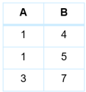
\includegraphics[width=0.45\textwidth,height=0.4\textheight,keepaspectratio]{../Lecture 5.2_artifacts/image_000008_161ab532df317073b117f157affb71c084307781898c1de51bc4b57e61d763d9.png}
        \end{center}
        \item On this instance, $A \rightarrow B$ does NOT hold, but $B \rightarrow A$ does hold. So we cannot have tuples like (2, 4), or (3, 5), or (4, 7) added to the current instance.
    \end{itemize}
\end{frame}

\begin{frame}{Functional Dependencies (3)}
    \begin{itemize}
        \item $K$ is a superkey for relation schema $R$ if and only if $K \rightarrow R$
        \item $K$ is a candidate key for $R$ if and only if
        \begin{itemize}
            \item $K \rightarrow R$ and
            \item for no $\alpha \subset K$, $\alpha \rightarrow R$
        \end{itemize}
        \item Functional dependencies allow us to express constraints that cannot be expressed using superkeys. Consider the schema:
        \begin{center}
        \texttt{inst\_dept(ID, name, salary, dept\_name, building, budget)}
        \end{center}
        \item We expect these functional dependencies to hold:
        \begin{center}
        \texttt{dept\_name $\rightarrow$ building} \\
        \texttt{dept\_name $\rightarrow$ budget} \\
        \texttt{ID $\rightarrow$ budget}
        \end{center}
        \item but would not expect the following to hold:
        \begin{center}
        \texttt{dept\_name $\rightarrow$ salary}
        \end{center}
    \end{itemize}
\end{frame}

\begin{frame}{Functional Dependencies (4)}
    \begin{itemize}
        \item We use functional dependencies to:
        \begin{itemize}
            \item test relations to see if they are legal under a given set of functional dependencies.
            \item $\triangleright$ If a relation $r$ is legal under a set $F$ of functional dependencies, we say that $r$ satisfies $F$
            \item specify constraints on the set of legal relations
            \item $\triangleright$ We say that $F$ holds on $R$ if all legal relations on $R$ satisfy the set of functional dependencies $F$
        \end{itemize}
        \item \textbf{Note}: A specific instance of a relation schema may satisfy a functional dependency even if the functional dependency does not hold on all legal instances
        \begin{itemize}
            \item For example, a specific instance of \texttt{instructor} may, by chance, satisfy \texttt{name $\rightarrow$ ID}
            \item In such cases we do not say that $F$ holds on $R$
        \end{itemize}
    \end{itemize}
\end{frame}

\begin{frame}{Functional Dependencies (5)}
    \begin{itemize}
        \item A functional dependency is trivial if it is satisfied by all instances of a relation
        \item Example:
        \begin{itemize}
            \item $\triangleright$ \texttt{ID, name $\rightarrow$ ID}
            \item $\triangleright$ \texttt{name $\rightarrow$ name}
        \end{itemize}
        \item In general, $\alpha \rightarrow \beta$ is trivial if $\beta \subseteq \alpha$.
    \end{itemize}
\end{frame}

\begin{frame}{Functional Dependencies (6)}
    \begin{itemize}
        \item Functional dependencies are:
        \begin{itemize}
            \item \texttt{StudentID $\rightarrow$ Semester}
            \item \texttt{StudentID, Lecture $\rightarrow$ TA}
            \item \texttt{\{StudentID, Lecture\} $\rightarrow$ \{TA, Semester\}}
        \end{itemize}
    \end{itemize}
    \begin{center}
    \begin{tabular}{|l|l|l|l|}
    \hline
    \textbf{StudentID} & \textbf{Semester} & \textbf{Lecture} & \textbf{TA} \\ \hline
    1234 & & Numerical Methods & John \\ 
    1221 & & Numerical Methods & Smith \\ 
    1234 & & Visual Computing & Bob \\ 
    1201 & & Numerical Methods & Peter \\ 
    1201 & & Physics II & Simon \\ \hline
    \end{tabular}
    \end{center}
\end{frame}

\begin{frame}{Functional Dependencies (7)}
    \begin{itemize}
        \item Functional dependencies are:
        \begin{itemize}
            \item \texttt{EmployeeID $\rightarrow$ EmployeeName}
            \item \texttt{EmployeeID $\rightarrow$ DepartmentID}
            \item \texttt{DepartmentID $\rightarrow$ DepartmentName}
        \end{itemize}
    \end{itemize}
    \begin{center}
    \begin{tabular}{|l|l|l|l|}
    \hline
    \textbf{Employee ID} & \textbf{Employee Name} & \textbf{Department ID} & \textbf{Department Name} \\ \hline
    0001 & John Doe & & Human Resources \\ 
    0002 & Jane Doe & & Marketing \\ 
    0003 & John Smith & & Human Resources \\ 
    0004 & Jane Goodall & & Sales \\ \hline
    \end{tabular}
    \end{center}
\end{frame}

\begin{frame}{Functional Dependencies (9): Closure of a Set of FDs}
    \begin{itemize}
        \item $F = \{A \rightarrow B, B \rightarrow C\}$
        \item $F^+ = \{A \rightarrow B, B \rightarrow C, A \rightarrow C\}$
    \end{itemize}
\end{frame}

\begin{frame}{Module Summary}
    \begin{itemize}
        \item Introduced the notion of Functional Dependencies
    \end{itemize}
    \vspace{2em}
    \begin{center}
    \small \textit{Slides used in this presentation are borrowed from \url{http://db-book.com/} with kind permission of the authors.} \\
    \small \textit{Edited and new slides are marked with 'PPD'.}
    \end{center}
\end{frame}

\end{document}
